\documentclass[10pt]{article}

% Just some packages I always include because they're useful
\usepackage{titlesec}
\usepackage[fleqn]{amsmath}
\usepackage{amsfonts}
\usepackage{algorithm}% http://ctan.org/pkg/algorithms
\usepackage{algpseudocode}% http://ctan.org/pkg/algorithmicx
\usepackage{hyperref}
\usepackage{verbatim}
\usepackage{textcomp}
\usepackage{a4wide}		% Always use this for A4 paper :)
\usepackage{lscape}


\usepackage{graphicx}
\graphicspath{ {images/} }

\title{Cloud Computing System Design\\Group 5}
\author{Tiago, Eddy, David Hoepelman}

\begin{document}

\maketitle

\section{Application selection}

Our use case is a library that has already digitized its paper collection. They find out they also want to OCR the collection so they can better search through it. Cost should be as low as possible, but there are little time constraints. One exception is new books, these should be digitized within a reasonable time. 

\section{System Design}

\subsection*{Global overview}

Our system uses a single master server that takes care of managment. Jobs (books) are distributed over workers, implemented as VMsx. To keep the cost low we use spot instances.

A diagram of our high-level system design can be found in Diagram \ref{diagram-hl-system-design}. We introduce the components:

%\begin{landscape}
%\begin{figure}[p]
%\centering
%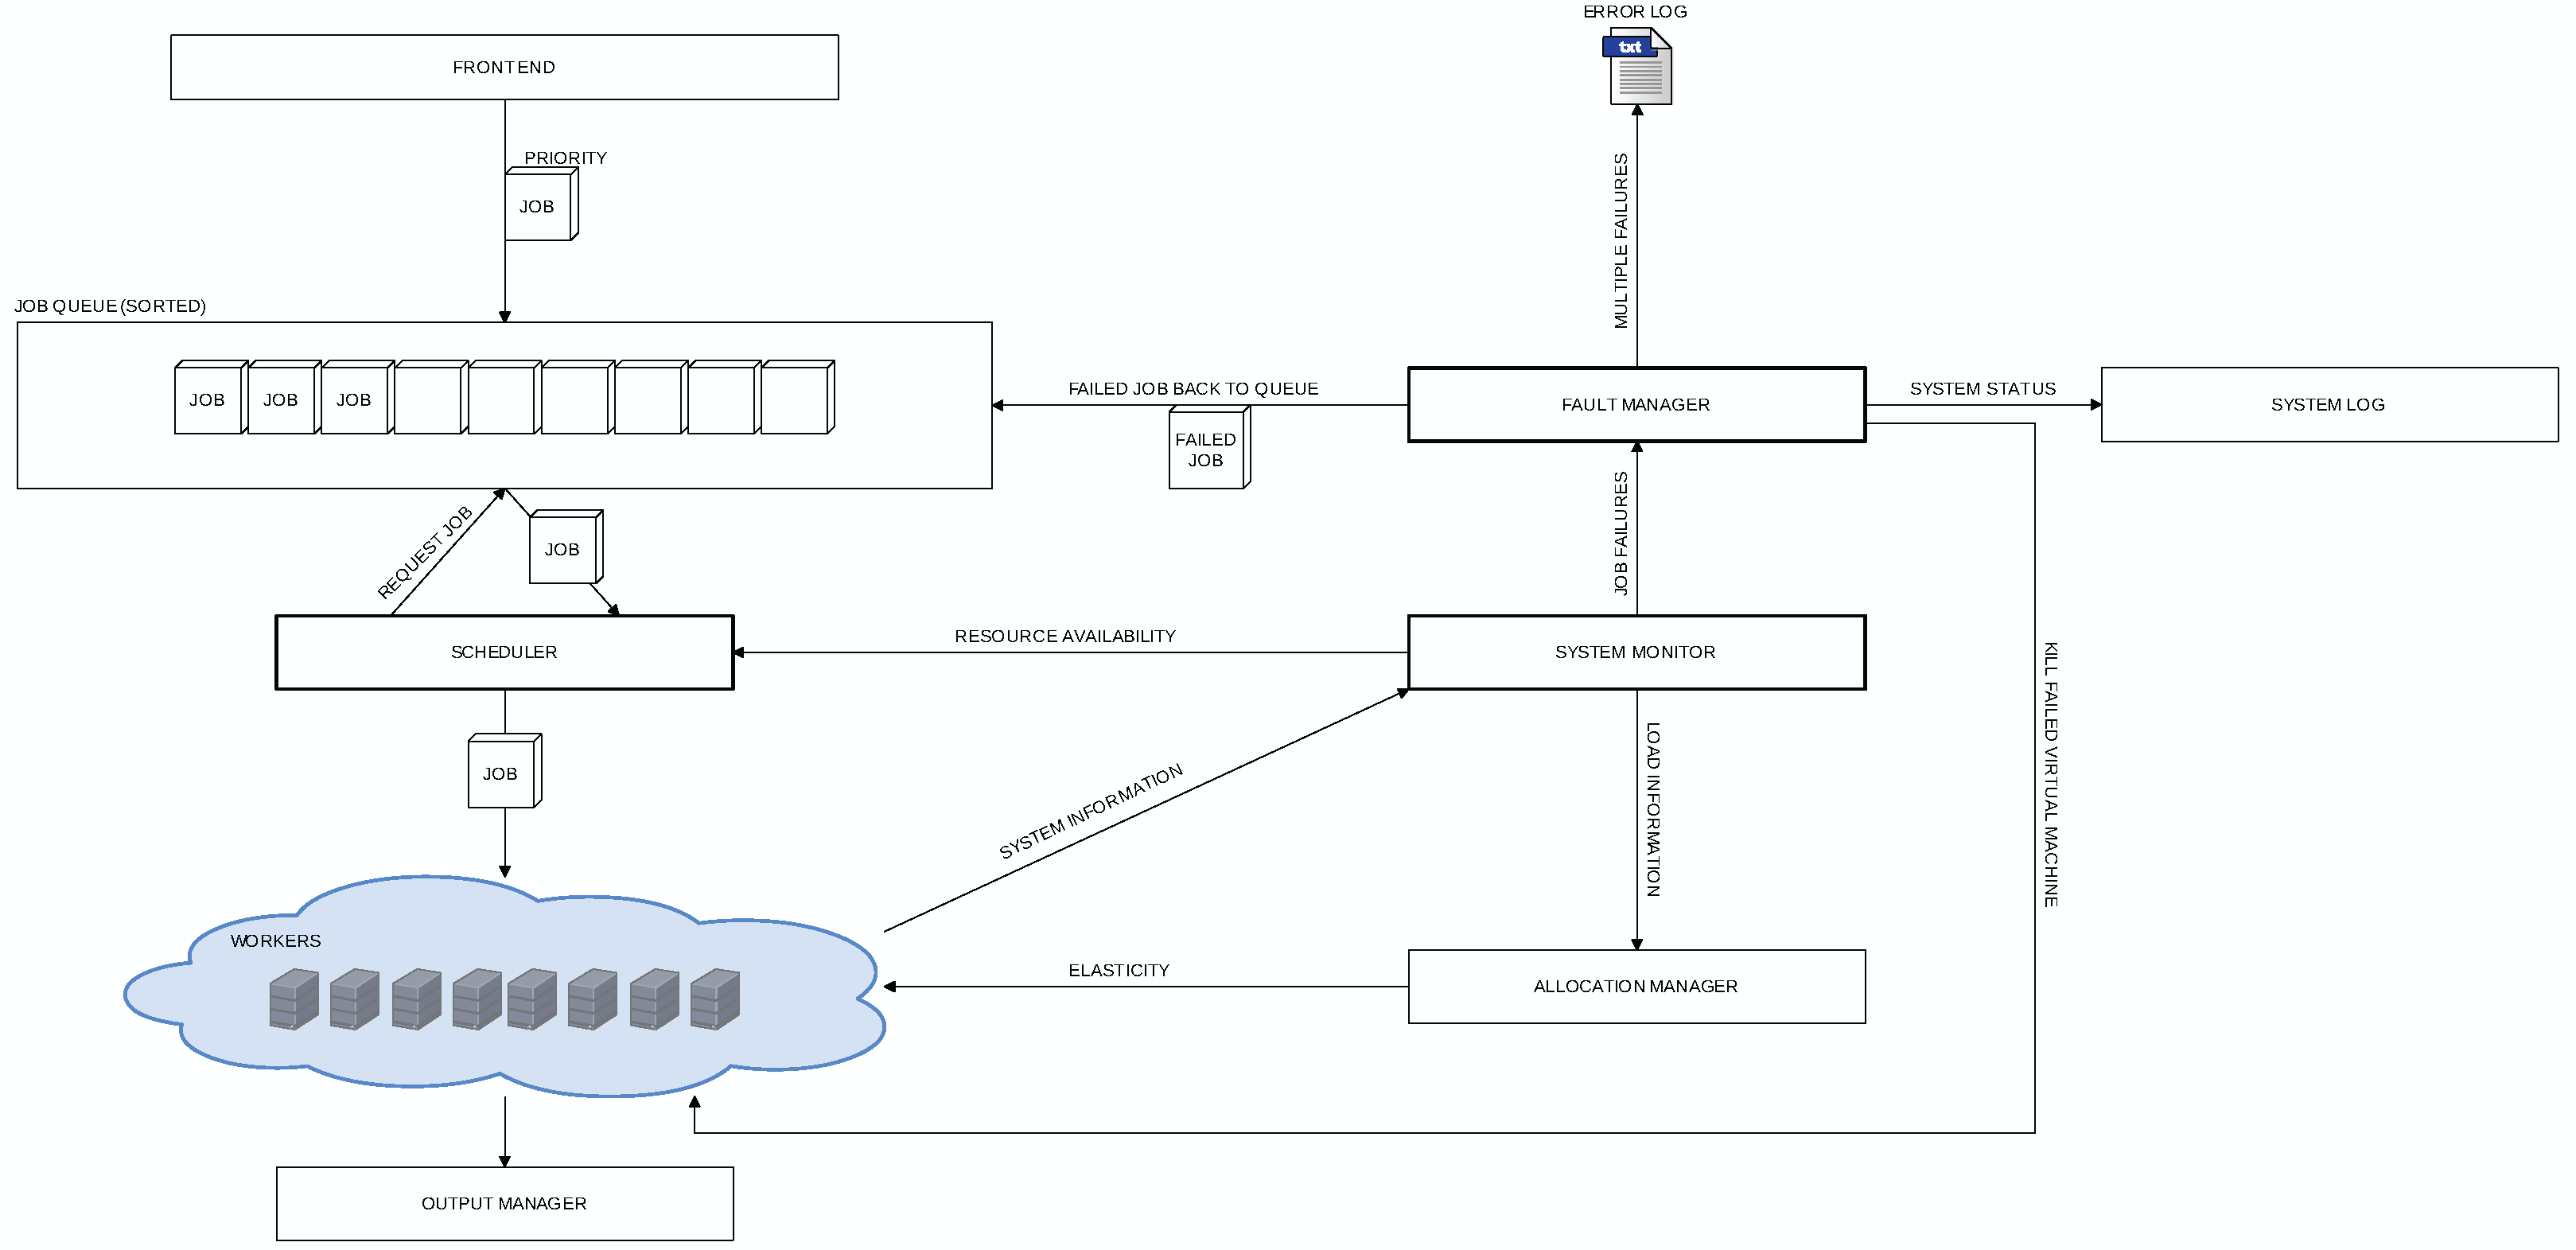
\includegraphics[width=\textwidth]{system_design_overview_png}
%\caption{Awesome Image}
%\label{fig:System Design Overview}
%\end{figure}
%\end{landscape}

\begin{itemize}

\item[Front-End] The front end \textbf{}is a web-interface where jobs can be submitted, and a priority can be assigned. Jobs are then added to the job queue. Different front ends can be made, we used a simple command-line script to add jobs.

\item[Job queue] The job queue holds jobs that still need to be processed and meta-information like priority and number of faults. It is sorted on priority.

\item[Job Scheduler]

The scheduler assigns jobs to workers and contains the logic for \textbf{load balacing}

\item[Workers]

A worker executes a job. They are implemented as Amazon EC2 instances running a common AMI having the open source OCR software Tesseract installed.

\item[Output Manager]

The output manager collects processed files and stores them so they can be retrieved by the user. \textbf{Durability} is possible based on global user preference.

\item[System Monitor]

The system monitor \textbf{monitors} characteristics of the workers which other components can use. These characteristics can be logged to use in analysis and benchmarking.

\item[Fault Manager]

The fault manager listens to fault information and handles accordingly. A failed job is resubmitted to the job queue and failing VMs are shutdown (if not already). A job that consistently fails is not resubmitted and logged in a dedicated log.

\item[Allocation Manager]

The Allocation Manager receives utilization information. Resources are allocated based on current throughput (compared to minimum required output). Spot instances are allocated when the price is low enough.

\end{itemize}

\subsection*{Resource managment}

\begin{itemize}
\item[Automation]

Most of the system is automated, only job submitting and inspecting faulty jobs is a manual task.

\item[Elasticity]

The \textbf{Allocation Manager} handles the allocation of resources and should be able to scale good. The master itself is not scaled.

\item[Performance]

The \textbf{Job Scheduler} takes care of load balancing.

\item[Reliability]

The system uses a master-slave architecture. The master contains all of the managment codes, while the slaves (workers) process the jobs. Reliability for the workers and jobs is provided by the \textbf{Fault Manager}, which handles failures in VMs and jobs.

Reliability for the master is not provided.

\item[Monitoring]

A dedicated monitoring subsystem monitors the workers and aggregates information, which can be logged if necessary.

\end{itemize}

\subsection*{System Policies}

\begin{itemize}

\item[Job Allocation]

Jobs can be give a priority by the user. Jobs will only be chosen by the scheduler when no higher-priority jobs are available. Jobs with the same priority are chosen in the order the were submitted to prevent starvation.

\item[Resource Allocation]

A configurable minimum throughput is maintained. There is no upper limit on allocated resources, if enough jobs are available and the price of spot instances is low enough.

\end{itemize}

\subsection*{Additional System Features}

\begin{itemize}

\item[Scheduling]

The solution focuses on efficient scheduling to minimize the total cost. This is done by the Allocation Manager which utilizes spot instances to keep the price as low as possible, while maintaining a minimal throughput. The user can configure this price/performance trade-off.

\item[Durability]

\emph{note: if time allows}. The systems saves the OCR'ed images compressed for collecting by the users. After a certain time results are relocated to long-term low-cast storage.

\end{itemize}

\end{document}